%-----------------------------------------------------------------------------------------------%
%
% Maret 2019
% Template Latex untuk Tugas Akhir Program Studi Sistem informasi ini
% dikembangkan oleh Inggih Permana (inggihjava@gmail.com)
%
% Template ini dikembangkan dari template yang dibuat oleh Andreas Febrian (Fasilkom UI 2003).
%
% Orang yang cerdas adalah orang yang paling banyak mengingat kematian.
%
%-----------------------------------------------------------------------------------------------%

%-----------------------------------------------------------------------------%
\chapter{\babLima}

\section{Implementasi Sistem}
Implementasi sistem merupakan tahap dimana sistem yang telah dirancang akan dijalankan. Implementasi sistem ini meliputi implementasi \textit{database}, implementasi \textit{routes}, implementasi \textit{model}, implementasi \textit{view}, dan implementasi \textit{controller}. Implementasi sistem ini dilakukan dengan menggabungkan 2 \textit{framework} yaitu Laravel dan Codeigniter.

\section{Batasan Implementasi}
Batasan implementasi Sistem Informasi Inventaris Laboratorium (SITARIS) dalam penelitian untuk Kerja Praktek ini adalah:
\begin{enumerate}
	\item Sistem yang dibangun memiliki \textit{platform} berbasis\textit{ Web}.
	\item Sistem yang dibangun memiliki hak akses seperti Admin, Kalab, Kaprodi, Sekprodi, dan Aslab.
	\item Menggunakan bahasa pemrograman PHP dengan \textit{framework} CodeIgniter dan \textit{database} MariaDB/PHPMyadmin.
	\item Sistem dapat menampilkan data barang, pendanaan, dokumentasi, peminjaman barang, peminjaman ruangan, \textit{maintenance}, pemusnahan barang, fakultas/lembaga, program studi/unit, gedung, ruangan, jadwal, dosen, mata kuliah dan pengguna.
\end{enumerate}

\section{Implementasi Perangkat Keras (\textit{Hardware})}
% -----------------------------------------------------------------------------%
Implementasi pada lingkungan \textit{hardware} adalah implementasi pada perangkat keras yang digunakan untuk menjalankan sistem informasi manajemen laboratorium. Implementasi \textit{hardware} yang digunakan dapat dilihat pada Tabel 5.1.

Minimum kebutuhan pada implementasi \textit{hardware} untuk menjalankan sistem informasi manajemen laboratorium adalah spesifikasi perangkat keras yang harus terpenuhi agar sistem dapat beroperasi secara optimal. Tabel 5.1. menyajikan daftar rinci dari komponen perangkat keras yang diperlukan dan spesifikasinya, yang mencakup prosesor, RAM, Hardisk, Monitor, dan perangkat masukan yang harus memenuhi standar minimum agar sistem berfungsi dengan baik.

\begin{table}[h]
	\centering
	\caption{Spesifikasi Perangkat Keras (\textit{Hardware})}
	\begin{tabular}{|l|l|}
		\hline
		\textbf{Komponen \textit{Hardware}} & \textbf{Spesifikasi}            \\ \hline
		Processor                           & Intel ® CoreTM i3-4160, 3.60GHz \\ \hline
		Memory (RAM)                        & 2 GB                            \\ \hline
		Hardisk (HDD)                       & 1 TB                            \\ \hline
		LCD                                 & Lenovo 17”                      \\ \hline
	\end{tabular}
\end{table}
\vspace{1cm}

\section{Implementasi Perangkat Lunak (\textit{Software})}
% -----------------------------------------------------------------------------%
Implementasi pada lingkungan \textit{software} adalah implementasi pada perangkat lunak yang digunakan untuk menjalankan sistem informasi inventaris laboratorium. Implementasi \textit{software} yang digunakan dapat dilihat pada Tabel 5.2.

\begin{table}[h]
	\centering
	\caption{Spesifikasi Perangkat Lunak (\textit{Software})}
	\begin{tabular}{|l|l|}
		\hline
		\textbf{Komponen \textit{Software}} & \textbf{Spesifikasi}              \\ \hline
		Sistem Operasi                      & Windows 7, 8, 10, dan 11          \\ \hline
		Browser                             & Google Chrome dan Mozilla Firefox \\ \hline
		Bahasa Pemrograman                  & PHP dan Javascript                \\ \hline
		Web \textit{Database}               & MariaDB                           \\ \hline
		\textit{Framework}                  & CodeIgniter 4                     \\ \hline
	\end{tabular}
\end{table}

\subsection{Implementasi \textit{Database}}
Pada implementasi \textit{database} ini nama yang digunakan adalah ”man\_lab”. Implemenasi \textit{database} ini terdapat beberapa tabel yang akan digunakan dalam sistem. Pembuatan \textit{database} dilakukan dengan menggunakan \textit{database} MariaDB. Tabel-tabel ini akan digunakan untuk menyimpan data-data yang diperlukan dalam sistem. Berikut adalah struktur tabel yang telah diintegrasikan dan digunakan dalam sistem ini dapat dilihat pada Gambar \ref{database-manlab}.

\begin{figure}
	\centering
	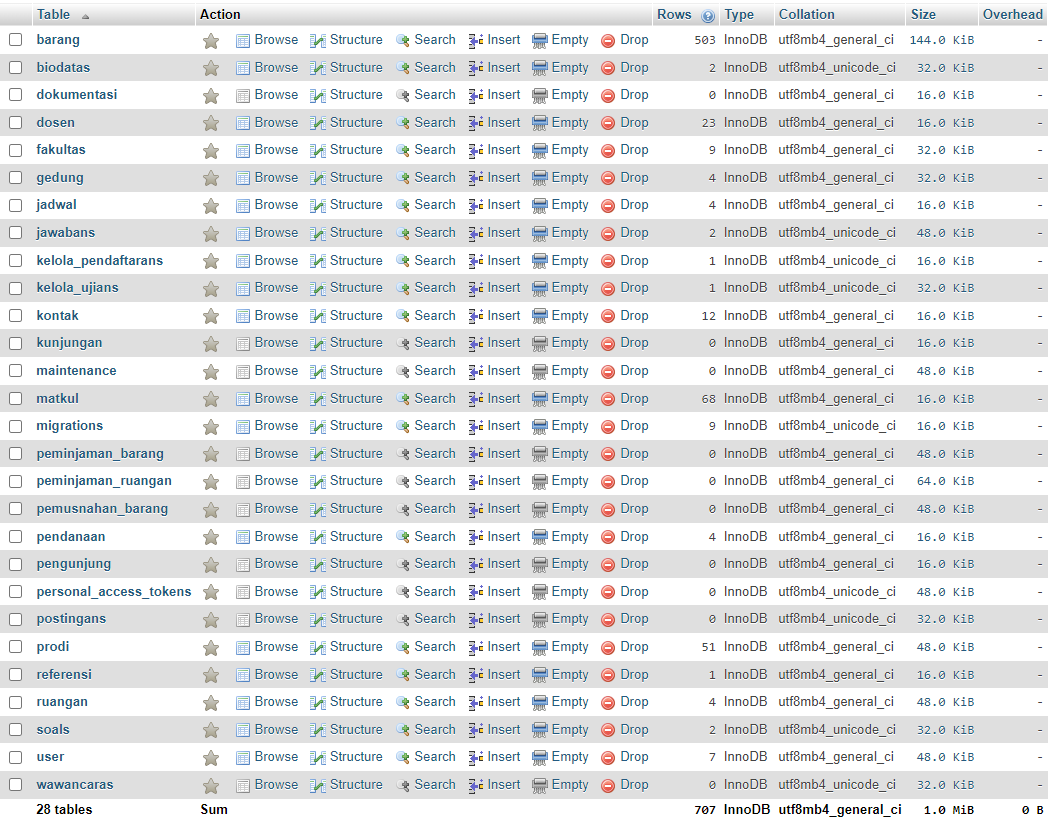
\includegraphics[width=1\textwidth]{konten/gambar/implementasi/database.png}
	\caption{\textit{Database}}
	\label{database-manlab}
\end{figure}

Pada pengembangan kali ini dilakukan penambahan tabel baru yaitu tabel "jadwal", "dosen", "mata kuliah", dan tabel  "biodatas", "users", "kelola pendaftarans", "kelola ujians", "postingans", "soals", jawabans", dan "wawancaras" sebagai tabel tambahan untuk integrasi sistem.

\begin{enumerate}

	\item Tabel Dosen dirancang untuk menyimpan informasi penting terkait dosen dalam sebuah sistem informasi. Kolom id\_dosen berfungsi sebagai kunci utama (primary key) yang memastikan setiap data dosen bersifat unik dan tidak terjadi duplikasi. Kolom nama\_dosen digunakan untuk mencatat nama lengkap dosen, sedangkan nip\_dosen menyimpan Nomor Induk Pegawai (NIP) sebagai identitas resmi dosen, jika tersedia. Untuk mencatat jenis kelamin, digunakan kolom jenis\_kelamin dengan opsi seperti "Laki-laki" atau "Perempuan". Informasi kontak dosen dicatat melalui kolom email\_dosen dan no\_hp, yang masing-masing menyimpan alamat email serta nomor handphone. Selain itu, kolom nidn digunakan untuk menyimpan Nomor Induk Dosen Nasional (NIDN) sebagai identitas unik dosen di tingkat nasional. Semua kolom ini dirancang untuk memastikan data dosen tersimpan secara lengkap, terstruktur, dan mudah diakses. Tampilan dapat dilihat pada Gambar \ref{tabel-Dosen}.

	      \begin{figure}
		      \centering
		      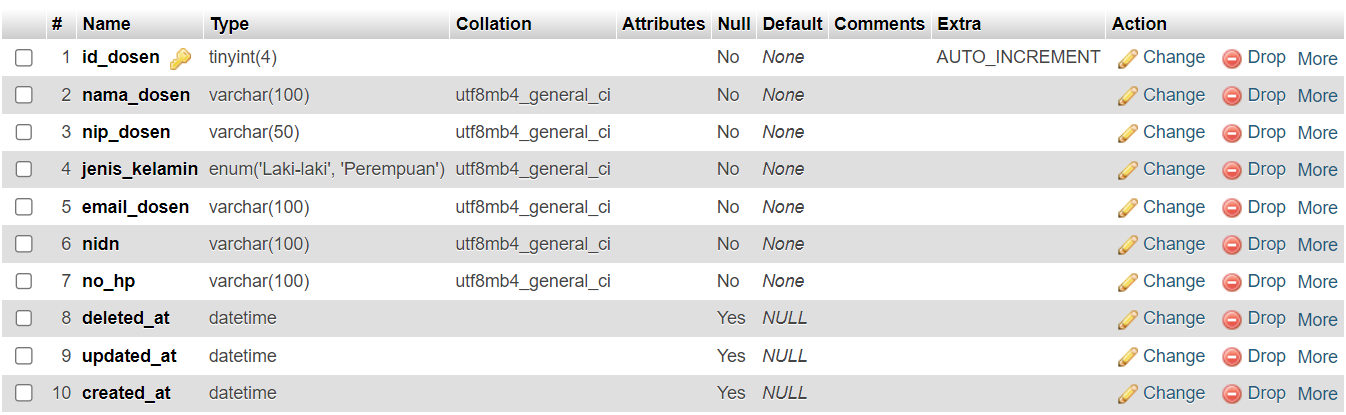
\includegraphics[width=0.82\textwidth]{konten/gambar/implementasi/tabel-dosen.png}
		      \caption{Tampilan \textit{Database} Tabel Dosen}
		      \label{tabel-Dosen}
	      \end{figure}


	\item Tabel Matkul digunakan untuk menyimpan informasi mengenai mata kuliah dalam sistem informasi akademik. Kolom id\_matkul berfungsi sebagai kunci utama (primary key) untuk mengidentifikasi setiap mata kuliah secara unik dan mencegah terjadinya duplikasi data. Kolom kode\_matkul menyimpan kode unik mata kuliah sebagai referensi singkat. Nama mata kuliah dicatat dalam kolom nama\_matkul untuk memberikan informasi deskriptif terkait mata kuliah tersebut. Kolom sks digunakan untuk mencatat jumlah Sistem Kredit Semester (SKS) dari mata kuliah, sedangkan semester mencatat pada semester berapa mata kuliah tersebut ditawarkan. Selain itu, kolom jenis\_matkul digunakan untuk mengklasifikasikan jenis mata kuliah, misalnya wajib dan pilihan. Struktur tabel ini dirancang untuk memastikan data terkait mata kuliah tersimpan secara terorganisasi dan mudah diakses sesuai kebutuhan. Tampilan dapat dilihat pada Gambar \ref{tabel-Matkul}.

	      \begin{figure}
		      \centering
		      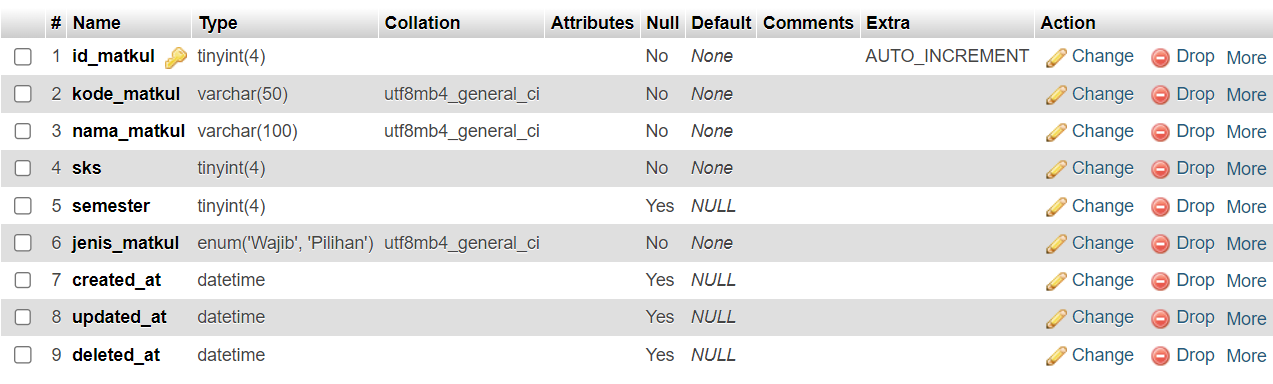
\includegraphics[width=0.82\textwidth]{konten/gambar/implementasi/tabel-matkul.png}
		      \caption{Tampilan \textit{Database} Tabel Matkul}
		      \label{tabel-Matkul}
	      \end{figure}

	\item Tabel Jadwal  terdiri dari kolom id\_jadwal yang menjadi kunci utama dari tabel tersebut yang digunakan sebagai penanda agar tidak terjadi duplikasi data, id\_ruangan digunakan untuk menunjukkan ruangan yang digunakan, id\_matkul digunakan untuk menunjukkan mata kuliah yang digunakan, id\_dosen digunakan untuk menunjukkan dosen yang mengajar, tanggal digunakan untuk menunjukkan tanggal pelaksanaan, hari digunakan untuk menunjukkan hari laboratorium digunakan, jam\_masuk dan jam\_keluar digunakan untuk menunjukkan jam digunakannya laboratorium, dan deskripsi digunakan untuk menunjukkan deskripsi dari jadwal tersebut. Tampilan dapat dilihat pada Gambar \ref{tabel-jadwal}.

	      \begin{figure}
		      \centering
		      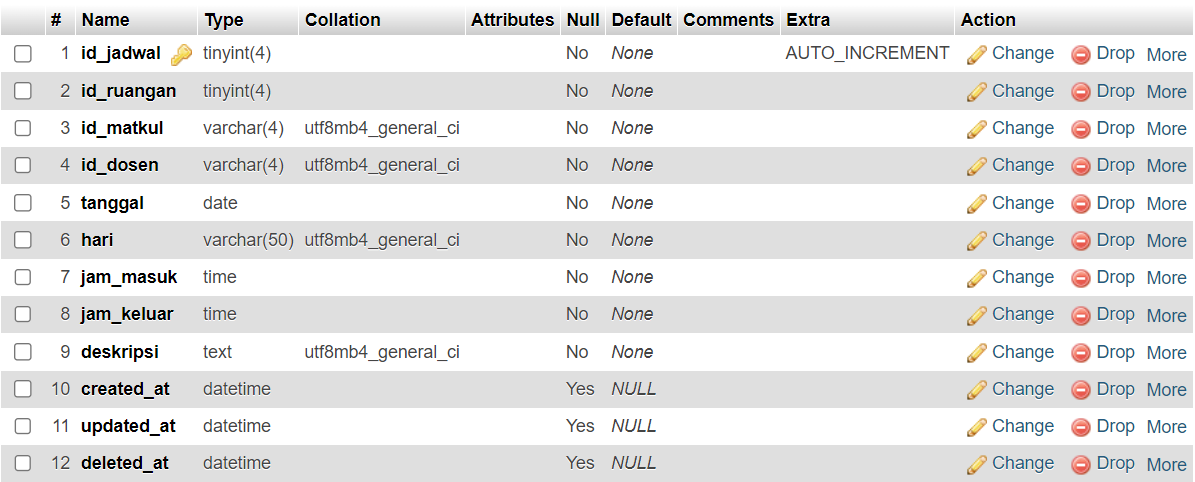
\includegraphics[width=0.82\textwidth]{konten/gambar/implementasi/tabel-jadwal.png}
		      \caption{Tampilan \textit{Database} Tabel Jadwal}
		      \label{tabel-jadwal}
	      \end{figure}

	\item Tabel Ruangan terdiri dari kolom id\_ruangan yang menjadi kunci utama dari tabel tersebut yang digunakan sebagai penanda agar tidak terjadi duplikasi data, id\_gedung menjadi kunci asing dalam tabel ruangan karena nama gedung diperlukan dalam pencatatan data ruangan, nama\_ruangan adalah kolom yang menyimpan nama ruangan yang dicatat, deskripsi\_ruangan menjelaskan detail tentang ruangan yang dicatat, gambar\_ruangan merupakan kolom untuk menyimpan data gambar dari ruangan yang dicatat. Tampilan dapat dilihat pada Gambar \ref{tabel-ruangan}.

	      \begin{figure}
		      \centering
		      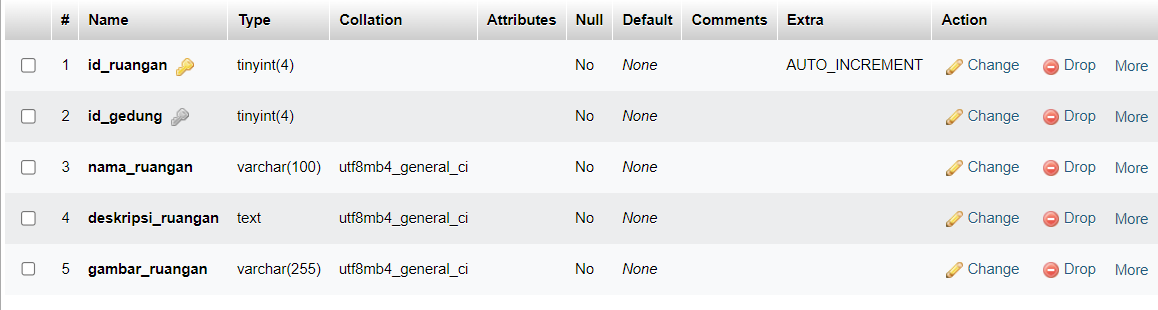
\includegraphics[width=0.82\linewidth]{konten//gambar/Tampilan database tabel ruangan.png}
		      \caption{Tampilan \textit{Database} Tabel Ruangan}
		      \label{fig:tabel-ruangan}
	      \end{figure}

	\item Tabel User terdiri dari kolom id\_user yang menjadi kunci utama dari tabel tersebut yang digunakan sebagai penanda agar tidak terjadi duplikasi data, nama merupakan kolom yang menyimpan nama pengguna, foto merupakan kolom untuk menyimpan foto profil pengguna, no\_identitas merupakan kolom yang digunakan untuk menyimpan data NIM, NIP, atau NIK dari pengguna, \textit{username} merupakan kolom yang digunakan untuk menyimpan \textit{username} pengguna, password\_hash merupakan kolom yang digunakan untuk menyimpan \textit{password} pengguna, email merupakan kolom yang digunakan untuk menyimpan email pengguna, role\_user merupakan kolom yang digunakan untuk menyimpan level akses pengguna. Tampilan dapat dilihat pada Gambar \ref{tabel-user}.

	      \begin{figure}
		      \centering
		      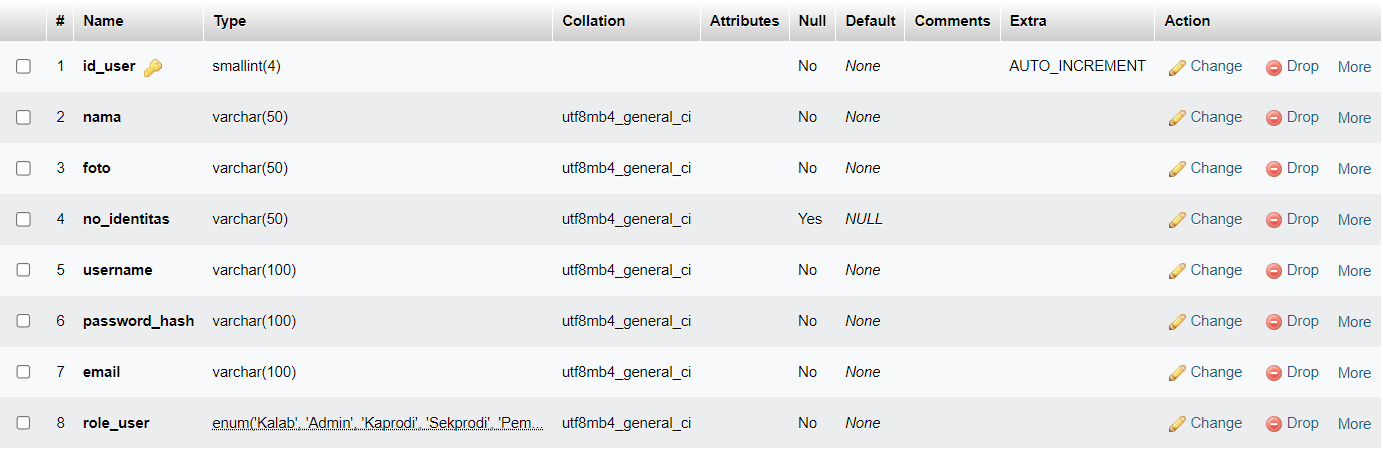
\includegraphics[width=0.82\linewidth]{konten//gambar/Tampilan database tabel user.png}
		      \caption{Tampilan \textit{Database} Tabel \textit{User}}
		      \label{fig:tabel-user}
	      \end{figure}
\end{enumerate}



\subsection{Implementasi \textit{Routes}}
\subsection{Implementasi \textit{Model}}
\subsection{Implementasi \textit{View}}
\subsection{Implementasi \textit{Controller}}
\section{Hasil Implementasi}
